\chapter{CHM compiler}

Our implementation of the CHM compiler uses preprocessing and postprocessing by gcc
with intermediate representation being pure C.

This allows us to focus on type inference and type checking instead of dealing with
meaning of the code, but the nature of this decision requires implementing some mangling
of names to give instances unique names.


\section{Language extensions}

The pure C language is extended by polytyped functions and structures and by
an addition of typeclasses which allow a way of overloading.

Polytyped functions allow to do the same algorithm on different data
which is useful in many situations, one such situation being iterating
through a list of items to do some action on them.

Polytyped structures can mainly serve as generic containers.
One example of this being % TODO: give an example

Type-classes together with polytyped functions allow us to give different
implementations to some functions depending on their parameters or return
types, this is especially useful in situations where the same implementation
for different data could lead to some slow-down or it could be even
impossible to make such an implementation.

% TODO: one example could be sorting where sorting numbers requires just a simple compare but in strings' case it required char-by-char iteration


\section{Type inference}

For the type inference we use thih, % TODO
but using it sensibly requires some modifications to be made and also a large
amount of pre/post-processing of the code.

\subsection{Typeclass preprocessing}

All typeclasses are just language construct, they are not manifested in the resulting code and thus they
count as a zero abstraction feature. There are some built-in typeclasses, % TODO
implicit typeclasses for each field of a structure (and a union) and then user=defined typeclasses.

Definitions of user-defined typeclasses are stored in the compiler as lists their methods are not important
for type-checking. All methods defined in type classes are replaced by functions with a constraint on the type
parameter of the typeclass. Then in instantiation the compiler checks whether they are methods and acts accordingly,
replacing them with the correct specialization, if indeed they are methods.

\subsection{Record fields}

Implementing support for record fields was difficult as in functional programming the way
record fields work in C has no real equivalent (pretty close being haskell's object notation or ML's records)

Record fields are implemented in such a way that we require the fields to be named differently
or to have the exact same type, all other situations are not specified as this cannot be
statically expressed in HM type system in any sensible way.

\xxx{Rict ze to ve FP nema obdobu takze na to aktualne dost kaslem.}

\subsection{Overloaded operators}
\xxx{...jen kdyz budes nejak resit operatory.}

\section{Monomorphization}

Monomorphization of functions is solved by recursive instantiation of symbols used in bodies of functions
starting from monotype functions.

Same applies to structures.

We will describe the process only on functions, but the principles of it carry to structures as well.

We start with monotype functions as we can already determine their monomorphic type. We replace all polymorphic
symbols in their definitions with unique symbols (distinct even if the original symbol was the same) with each
assigned a new unique type variable. We run the inference algorithm on this rewritten definition and then if
we successfully determined each monotype (for example we cannot if we have a type variable `a' in the declaration `a x;'
and `a' is never used again) we instantiate each of the original symbols given the new inferred type (unless we have done already).

\subsection{Overloading resolution}

Overloading is resolved by remembering which symbols belong to methods (or type families), then we look with which type of an
instance it can unify to determine which definition of the function (structure) we want to instantiate.

\subsection{Recursion limits}

It is indeterminable whether instantiation of something continues forever. We can prove this using post correspondence problem % FIXME: prove it

So there is a limit of type depth set to 500 (this limit shouldn't affect any sensible program).
% FIXME: Changing this limit is possible by adding an option --type-depth=N to the compiler (it can be also used to make stricter constraint as well).
If some type exceeds this limit, an compilation error will be outputted stating what the compiler was instantiating
at that time.

\subsection{Comparison to C++ template instantiation}

One could say this project just mirrors template instantiation from C++, but any such resemblance is just
superficial, C++ template instantiation is not strict in type signatures and different instances can have
non-matching types.

One example of this would be:

template<typename>
struct function_type;

template<>
struct function_type<int> { using return_type = int; using parameter_type = int; };

template<>
struct function_type<int*> { using return_type = int; using parameter_type = int*; };

template<>
struct function_type<int**> { using return_type = int*; using parameter_type = int; };

template<typename T>
typename function_type<T>::return_type function(typename function_type<T>::parameter_type);

template<>
int function<int>(int value) { return value; }

template<>
int function<int*>(int *value) { return *value; }

template<>
int *function<int**>(int value) { return &value; }

C++ allows different instances to have the same type signature which can make any type inference or type deduction
impossible.

One more difference is that C++ allows function overloading. % TODO: write about the paper linked by mirek

The instantiation in CHM follows inferred types by the HM type system.

\section{Code output}

The CHM compiler outputs gcc-compilable code which interprets the CHM code without any runtime overhead. % TODO: or at least so I hope

There are options allowing the user to see the inner haskell representation of the CHM code (it blurs some of the semantics
unnecessary for type inference and leaves others to facilitate the readability of it), this can be used for debugging
the compiler implementations. % FIXME: list the options (unimplemented yet)

It should be noted that names of symbols of polytype functions actually used in the C interpretation of the CHM code do not match
their CHM counterparts which currently complicates debugging of CHM programs (this however can be solved easily on the debugger side).

\chapter{Results and discussion}


Instead, try some of the following:
\begin{itemize}
\item State a hypothesis and prove it statistically
\item Show plots with measurements that you did to prove your results (e.g. speedup). Use either \texttt{R} and \texttt{ggplot}, or Python with \texttt{matplotlib} to generate the plots.\footnote{Honestly, the plots from \texttt{ggplot} look \underline{much} better.} Save them as PDF to avoid printing pixels (as in ).
\item Compare with other similar software/theses/authors/results, if possible
\item Show example source code (e.g. for demonstrating how easily your results can be used)
\item Include a `toy problem' for demonstrating the basic functionality of your approach and detail all important properties and results on that
\item Include clear pictures of `inputs' and `outputs' of all your algorithms, if applicable
\end{itemize}

\begin{figure}
\centering
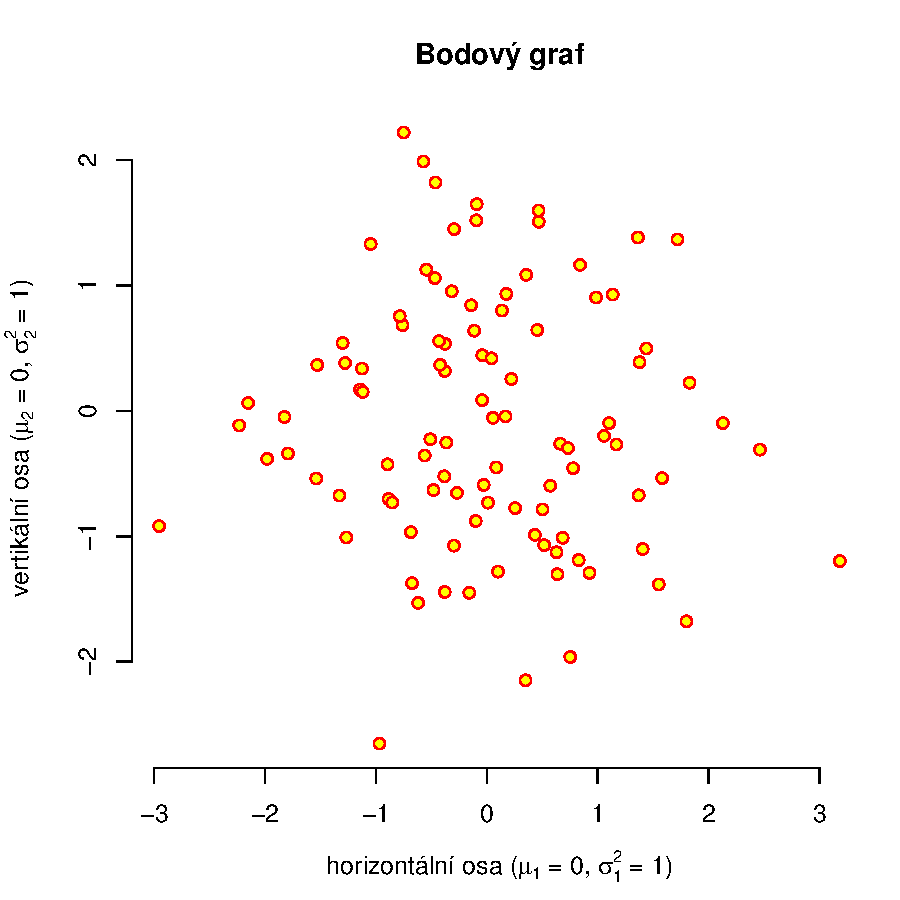
\includegraphics[width=.6\linewidth]{img/ukazka-obr01.pdf}
\caption{This caption is a friendly reminder to never insert figures ``in text,'' without a floating environment}
\label{fig:f}
\end{figure}

It is sometimes convenient (even recommended by some journals, including Cell) to name the results sub-sections so that they state what exactly has been achieved. Examples follow.

\section{SuperProgram is faster than OldAlgorithm}
\subsection{Scalability estimation}
\subsection{Precision of the results}
\section{Weird theorem is proven by induction}
\section{Amount of code reduced by CodeRedTool}
\subsection{Example}
\subsection{Performance on real codebases}
\section{NeuroticHelper improves neural network learning}

\section{What is a discussion?}
After you present the results and show that your contribution works, it is important to \emph{interpret} them, showing what they mean for the more general public.

Separate discussion sections are common in life sciences where ambiguity is common and intuition is sometimes the only thing that the authors have; exact sciences and mathematicians do not use them as often. Despite of that, it is nice to precisely set your output into the existing environment, answering:
\begin{itemize}
\item What is the potential application of the result?
\item Does the result solve a problem that other people encountered?
\item Did the results point to any new (surprising) facts?
\item Why is the result important for your future work (or work of anyone other)?
\item Can the results be used to replace (and improve) anything that is used currently?
\end{itemize}

If you do not know the answers, you may want to ask the supervisor. Also, do not worry if the discussion section is half-empty or completely pointless; you may remove it completely without much consequence. It is just a bachelor thesis, not a world-saving avenger thesis.
